\documentclass[12pt]{report}
\usepackage[utf8]{inputenc}
\usepackage[french]{babel}
\usepackage[T1]{fontenc}
\usepackage{amsmath}
\usepackage{amsfonts}
\usepackage{amssymb}
\usepackage{graphicx}
\usepackage{titlesec}
\usepackage{caption}
\usepackage{titling}
\usepackage{booktabs}
\usepackage{enumitem}
\usepackage{eurosym}
\usepackage{epigraph}
\usepackage{hyperref}
\usepackage{fontspec}
\usepackage{ragged2e}
\usepackage{parskip}
\usepackage{wrapfig}
\usepackage{calc}
\usepackage{float}
\usepackage{setspace}

\onehalfspace

\graphicspath{ {img/} }
\setlength{\droptitle}{-10em}
\setlength{\parskip}{2em}
\titleformat{\chapter}[hang]{\normalfont\huge\bfseries}{\thechapter. }{0em}{}

\begin{document}

\title{
	{\Huge Projet OCR}\\
	\vspace{2em}
	{\Huge Rapport de projet}\\
	{\large Wizard Neurons}
}
\author{
	Antoine Gonzalez\\
	Cédric Parpet
	\and
	Louis Le Gatt\\
	Jérémy Salfati}
\date{
	\vspace{15em}
	{Dossier Projet Informatique\\
	Info-Spé EPITA\\
	Décembre 2018}
}

\maketitle
\newpage
\newpage
\tableofcontents

\chapter{Introduction}

Le semestre touche à sa fin, et il en va de même pour notre projet. Cet OCR aura été un véritable challenge. Mais avec beaucoup d'effort, de persévérence, et de manque de sommeil, notre groupe a finalement pu venir à bout de ce projet.

L'aventure n'aura pas été simple. Toutes les parties de ce projet représentaient quelque chose de nouveau pour nous. Nous n'avions jamais pu manipuler d'interface graphique auparavant, sauf peut être lors du projet du semestre précédent ; le concept de réseau de neurones était totalement nouveau, et enfin réussir à organiser le traitement et découpage d'une image tout en liant correctement toutes les parties de ce programme aura été un véritable casse tête. De plus, le langage C est loin d'être le plus simple à prendre en main, et la gestion manuelle de la mémoire nous a apporté plus de problèmes que de possibilités.

\newpage

Toutefois, ces problèmes ont pû être surmontés, et nous disposons à présent d'un réseau de neurones capable d'apprendre l'alphabet avec des résultats corrects, d'une interface graphique fonctionnelle, d'un découpage de l'image performant et d'un traitement adapté au problème de la reconnaissance de texte.

Dans ce rapport de projet, nous reviendrons sur les différentes étapes de la réalisation de notre OCR, son fonctionnement, sur les difficultés rencontrées, et enfin sur ce qu'il nous a apporté au niveau personnel.

\begin{figure}
    \centering
    
\includegraphics[width=0.6\textwidth]{project_mood_S2}
    \caption*{\textit{Calvin and Hobbes}, Bill Watterson}
\end{figure}

\chapter{Répartition des tâches}

Commençons par un bref rappel de la répartition des tâches au sein du groupe:

\begin{center}
    \begin{tabular}{@{} l *4c @{}}
        \toprule
        \multicolumn{1}{c}{}    & \textbf{Antoine}  & \textbf{Louis}  & \textbf{Cédric} & \textbf{Jérémy} \\ 
        \midrule
        Chargement de l'image & & & & X \\
        Traitement de l'image & & X & & \\
        Découpage de l'image & & & X & \\
        Réseau Neuronal & X & & & \\
        Sauvegarde des résultats & & & & X \\
        Interface Utilisateur & & & & X \\
        \bottomrule
    \end{tabular}
\end{center}


Notre organisation n'a pas évolué depuis la première soutenance: Antoine s'occupe du réseau neuronal, Louis du traitement et de la manipulation de l'image avec la SDL, Cédric de la segmentation du texte et de sa reconstruction, et enfin Jérémy de l'interface utilisateur. L'interface utilisateur doit bien entendu se charger de lancer la reconnaissance de texte depuis l'image choisie.

\chapter{Diagramme Fonctionnel}

Afin que chaque membre comprenne parfaitement ce qui est attendu de sa partie et comment elle devra interagir avec celle des autres membres, nous avons réalisé un diagramme fonctionnel de l'OCR. On peut y voir le déroulement de son éxecution, du moment où l'utilisateur charge une image, au moment où le texte détecté est affiché et enrgistré \textit{(voir figure ci-dessous)}.

Comme on peut le voir, chaque partie interagit de manière simple avec le reste, et possède un but bien défini. Chaque morceau de l'OCR n'appelle qu'une unique autre partie, ce qui limite les erreurs potentielles d'appels croisés entre les multiples fonctions. Chaque membre du groupe n'a donc qu'à penser à une seule autre partie. Il lui suffit de spécifier quel type de valeur il attend en retour, et quel type de valeur il est capable d'envoyer. La partie suivante n'a qu'à s'adapter à ces règles, et faire de même.

\begin{figure}[H]
    \centering
    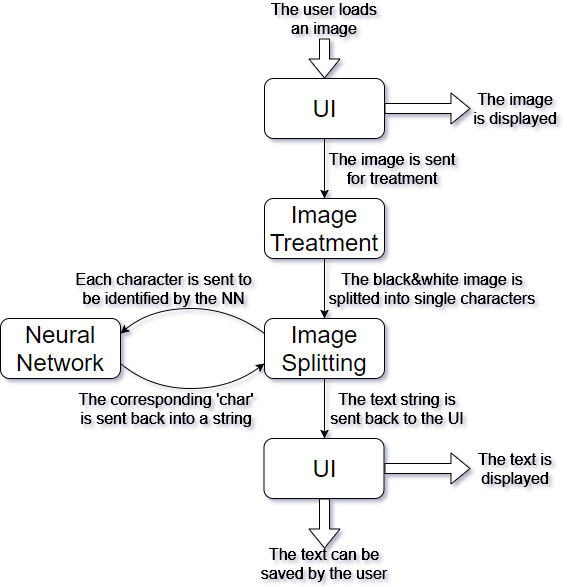
\includegraphics[width=1\textwidth]{OCR_functionnal_diagram}
    \caption{Functional diagram}
\end{figure}

\chapter{Déroulement du projet}

\section{Traitement de l'image (Louis)}

Mon travail sur cet OCR était principalement la réalisation du traitement de l’image. Pour cela j’ai utilisé la bibliothèque SDL qui permet le traitement des images de manière simple. Il s’agissait de la bibliothèque la plus simple et la plus efficace à mes yeux pour réaliser le travail demandé sur le traitement de l’image pour cet OCR. 
Les consignes étaient claires pour le traitement de l’image. Il fallait supprimer les couleurs et renvoyer une image en noir et blanc sans perte de donnée afin de ne pas ralentir le réseau de neurones ou la segmentation dans leur travail. De plus j’ai décidé d’ajouter une fonction de réduction de bruit sur l’image et une fonction permettant de redimensionner les différents caractères en sortie de la segmentation.
Ainsi le procédé pour le traitement de l’image est le suivant: tout d’abord appliquer un filtre de teinte de gris sur l’image, calculer la moyenne de la valeur des pixels de l’image pour obtenir un « seuil », et enfin appliquer un filtre noir et blanc à l’image pour obtenir une image binaire.

\begin{figure}[H]
    \centering
    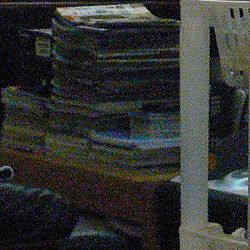
\includegraphics[width=0.5\textwidth]{noise}
    \caption{Original image}
\end{figure}

Commençons par la réalisation des différentes fonctions de traitement de l’image.
Pour ces fonctions j’ai commencé par apprendre les différentes manières de coder en C qui me seront utile pour cette partie. Je me suis ensuite documenté sur différents algorithmes utilisant la bibliothèque SDL afin de m’en inspirer et de comprendre le fonctionnement de cette bibliothèque. J’ai finalement commencé par coder les fonctions permettant de passer l’image en noir et blanc et en teinte de gris. J’ai ainsi tout de suite eu besoin de différentes fonctions permettant d’accéder à des pixels et de les modifier. Pour cela j’ai utilisé deux fonctions vues en travaux pratiques : getpixel et putpixel qui permettent, pour la première de récupérer la valeur d’un pixel donné et pour l’autre de placer un pixel sur une surface à une coordonnée x,y choisie. J’ai ainsi décidé d’écrire ces fonctions dans un fichier autre que celui sur lequel j’ai réalisé les différentes fonctions de traitement de l’image car les opérations sur les pixels peuvent s’avérer utiles et pratiques pour les autres membres du groupe.

\newpage

Pour la fonction de noir et blanc je n’ai pas tout de suite pensé à calculer un seuil sur l’image. En effet je pensais que le fait de simplement mettre un seuil à 128 (valeur du pixel) pour tous les pixels de l’image serait suffisant. Malheureusement dans plusieurs cas comme par exemple dans le cas où le fond de l’image et le texte sont d’une couleur proche le texte disparaissait et le travail de la segmentation devenait impossible. J’ai alors décidé qu’il fallait calculer un seuil différent pour chaque image en fonction de la couleur moyenne des pixels de celle-ci. Ainsi pour éviter de tester les valeurs de chacune des composantes des différents pixels (rouge, bleue, verte) j’ai décidé d’appliquer un filtre de teinte gris à l’image. En effet le filtre pour la teinte de gris applique à chacune des composantes des pixels la même valeur. C’est-à-dire que les valeurs du rouge, du bleu et du vert sont identiques. Cela permet à la fonction passant l’image en noir et blanc de ne tester qu’une des trois composantes à chaque pixel donnant un gain de temps important sur la totalité de l’image. 

\begin{figure}[H]
    \centering
    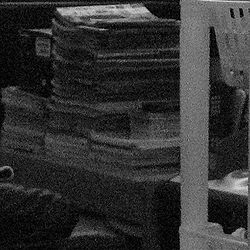
\includegraphics[width=0.5\textwidth]{grayscale}
    \caption{Grayscale}
\end{figure}

\newpage

Pour le calcul du seuil je réalise un simple parcours de l’image et j’applique le calcul de la moyenne de la totalité des pixels. J’obtiens ainsi la valeur d’un pixel moyen de l’image. La fonction noir et blanc utilise alors ce seuil afin de décider si le pixel doit devenir noir ou blanc en réalisant un simple test sur l’une des trois composantes du pixel. Suite à ce test le pixel devient noir ou blanc.

Mes camarades de projet souhaitaient pouvoir sauvegarder les images. J’ai alors réalisé quelques recherches afin de trouver un moyen simple de sauvegarder cette image. SDL ayant une fonction prédéfinie pour cette sauvegarde je l’ai utilisé. De plus il fallait pouvoir copier l’image envoyée par l’utilisateur afin de ne pas réaliser les différents traitements de l’image directement sur l’image de l’utilisateur. Dans le but de restituer à l’utilisateur son image sans aucun changement de nom ou de structure.

J’ai finalement décidé d’ajouter une fonctionnalité supplémentaire au traitement de l’image. En réalisant quelques recherches je me suis rendu compte qu’un des traitements pouvant être intéressant pour notre OCR était la réduction de bruit. Après de nombreuses recherches à travers des méthodes plus ou moins complexes afin de réduire le bruit sur une image je me suis arrêté sur une méthode nommé le filtre médian. Ce filtre médian est plutôt simple à comprendre. En effet il suffit de parcourir l’image pixel par pixel et d’observer pour chacun des pixels ses pixels voisins. Il suffit ensuite de réaliser une liste de ces différents pixels en y intégrant leur valeur numérique correspondant à leur couleur. Finalement cet algorithme trie cette liste en ordre croissant en utilisant un bubblesort. Il suffit ensuite de trouver la valeur du milieu de cette liste qui devient la nouvelle valeur du pixel. 

\newpage

Ainsi chaque pixel est une moyenne des pixels voisins à celui-ci ce qui permet de supprimer le bruit de l’image car les pixels de "bruit" ont une valeur qui ne sera jamais la valeur médiane de ses pixels voisins. Ainsi le pixel de "bruit" se retrouve supprimé de l’image.

\begin{figure}[H]
    \centering
    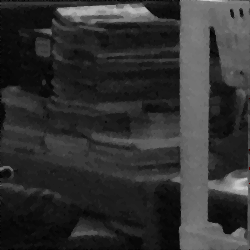
\includegraphics[width=0.5\textwidth]{noiseless_grayscale}
    \caption{Grayscale without noise}
\end{figure}

Cependant après de nombreux essais sur différentes images, je me suis rendu compte que la qualité des caractères se retrouvait détériorée à la suite de l’appel à cette fonction. En effet en appliquant ce filtre les lettres présentes sur les images se retrouvent déformées. Cependant cette fonction marche sur des images présentant du bruit malgré la déformation des lettres. J’ai ainsi essayé d’améliorer cette fonction afin de la rendre utilisable pour notre OCR et donc qu’elle ne déforme pas les lettres mais qu’elle continue d’être aussi efficace pour supprimer le bruit des images. 

\newpage

Après de nombreux essais je n’ai pas réussi à rendre cette fonction utilisable. Elle pourrait cependant se rendre utile si nous avions pu réaliser un bouton sur l’interface graphique sur lequel l’utilisateur aurait pu appuyer si la quantité de bruit sur l’image était suffisante pour rendre la segmentation inefficace.

Antoine, qui s’occupait du réseau de neurones m’a demandé de réaliser une fonction permettant de redimensionner une image. Comme je l’ai déjà dit auparavant cette fonction a pour but de renvoyer une image de taille correcte pour que le réseau de neurones puisse la reconnaitre. Ainsi j’ai tout d’abord essayé de créer ma propre fonction qui redimensionnerait notre image donnée en paramètre. Puis après quelques recherches et plusieurs conversations avec d’autres membres d’autres projets j’ai appris qu’il existait une fonction SDL permettant de redimensionner son image. J’ai donc utilisé cette fonction.

Le traitement de l’image est donc entièrement fonctionnel bien que la réduction du bruit ne puisse être utilisée sous cette forme. L’image est donc entièrement traitée, on lui supprime ses couleurs en perdant le moins d’information possible, on l’envoie à la segmentation puis on redimensionne les caractères en sortie pour finalement les donner au réseau de neurones.

\newpage

\section{Segmentation de l'image (Cédric)}

Pour ce projet, je me suis porté volontaire pour m'occuper de la partie concernant la segmentation. J'ai utilisé la bibliothèque SDL afin de manipuler les images que l'on utilisait.

Lors de la première soutenance j'avais développé une segmentation itérative qui fonctionnait correctement. Cependant j'avais prévu d'en refaire une de manière récursive, notamment grâce à l'algorithme \textit{recursive XY cut}, avec pour objectif de pouvoir prendre en compte un découpage en blocs afin de séparer correctement les blocs de textes entre eux, mais aussi avec l'objectif de pouvoir restituer les espaces et les retours à la ligne de manière plus efficace. Malheureusement je n'ai pas réussi à faire cette segmentation récursive et nous avons décidé de garder la fonction itérative. 

La fonction récursive devait fonctionner ainsi : On crée un histogramme des pixels noirs et blancs des lignes et des colonnes puis on parcourt cette liste pour trouver le plus grand espace vide (sans pixels noirs). On compare ensuite le plus grand espace vide des colonnes entre les colonnes et les lignes afin de savoir où couper. On continue ainsi de suite jusqu'à ce qu'il n'y ait plus de lignes sans pixels et on crée une image à partir du rectangle obtenu. Chaque image obtenue de cette manière ne contient que le caractère à donner à la fonction de redimensionnement.
Cependant le temps passé à essayer d'implémenter la récursion n'aura pas été inutile car j'ai pu réutiliser la création des histogrammes pour analyser mes images plus facilement. 

\newpage

Cela aura notamment été utile pour la fonction qui enlève les bords blancs d'une image dont je parlerai plus tard car si la fonction récursive devait le faire automatiquement, la fonction itérative ne le fait pas et cela se révélera nécessaire pour reconnaître efficacement le caractère par le réseau de neurones.

La fonction de segmentation va récupérer des coordonnées x,y pour déterminer un rectangle dans lequel se situera un caractère. Il fonctionne ainsi : 
\begin{itemize}[label=\textbullet]
	\item Nous parcourons l'image ligne par ligne puis lorsque l'on détecte un pixel on récupère l'indice de la ligne.
	\item Nous continuons de parcourir les lignes jusqu'à ce qu'on trouve une ligne sans pixel.
	\item Nous récupérons donc l'indice de la ligne d'avant et on a ainsi l'intervalle dans laquelle on a une ligne de texte.
	\item Nous parcourons les colonnes de manière similaire, entre l'intervalle correspondant à la ligne de texte, pour obtenir deux indices de plus. Et grâce à ces quatre données on peut créer un carré dans lequel se situe un caractère.
	\item Nous allons ensuite créer une image correspondant au contenu de ce rectangle grâce aux fonctions prédéfinies de SDL, puis couper les potentiels bords blancs avant de la redimensionner en une image 10 par 10 et ensuite de le donner au réseau de neurones. 
	\item Nous récupérons ensuite le caractère et nous l'ajoutons à la string que renverra la segmentation et initialisé à '''' .
	\item Nous parcourons ensuite les autres colonnes jusqu'à la fin de la ligne de texte et on répète le processus depuis le début pour le reste des lignes de pixels de l'image.
	\item Lorsque l'on parcourt les colonnes et que l'on détecte une colonne sans pixels noirs, on incrémente une variable pour calculer l'espace. 
	\item Une fois une colonne avec pixel noir trouvée, nous ajoutons un espace ou une tabulation (en fonction de la longueur) à la liste puis on réinitialise le compteur à 0.
\end{itemize}

\begin{figure}
    \centering
    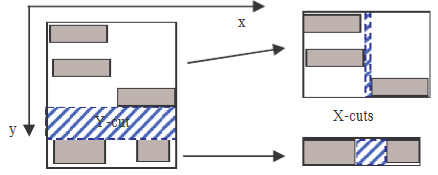
\includegraphics[width=1\textwidth]{Image_segmentation}
    \caption{Image segmentation}
\end{figure}

\begin{figure}
    \centering
    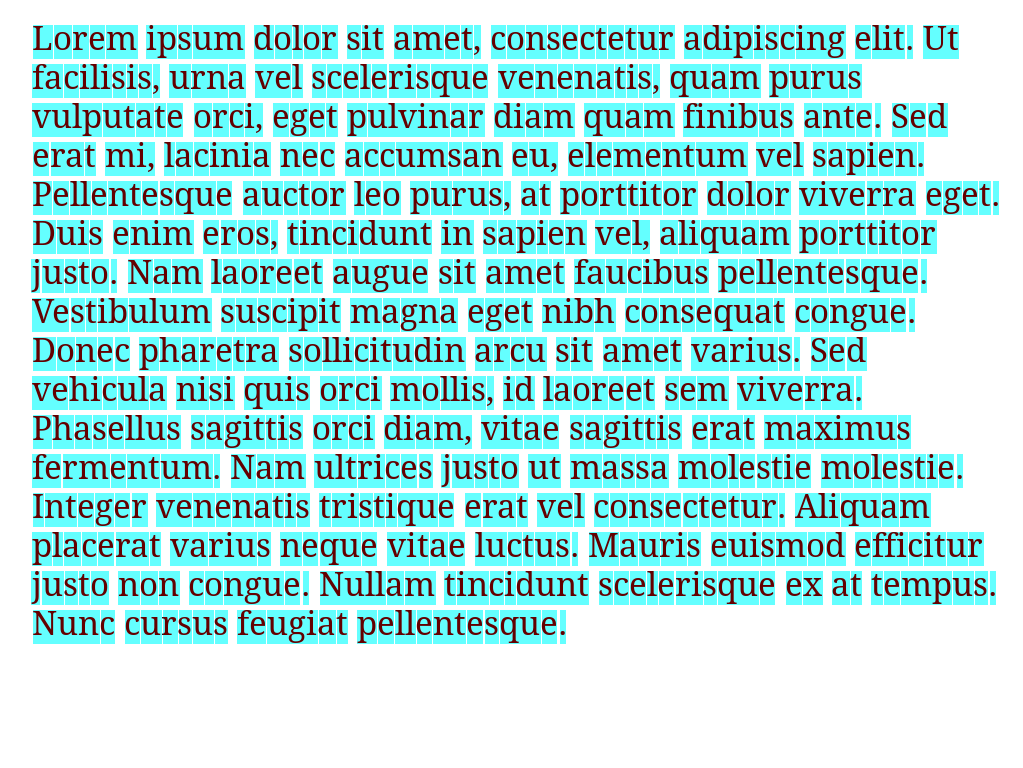
\includegraphics[width=0.8\textwidth]{Seg_example_2}
    \caption{Example 2}
\end{figure}

La fonction permettant de couper les bordures blanches d'une image se trouve en réalité très utile : Les rectangles créés par la segmentation ont une épaisseur qui correspond à l'épaisseur du caractère, mais leur hauteur correspond à celle de la ligne de texte. Par exemple s'il y a un "l" et un "e" sur la même ligne de texte, la hauteur de leur rectangle respectif les contenant auront une largeur différente mais la même hauteur. Lors du redimensionnement de l'image, le "e" sera moins bien déformé et le réseau de neurones risque de pas le reconnaître. Sans les bordures blanches la lettre sera mieux redimensionnée et le réseau la reconnaîtra.

\newpage

La fonction est très simple et fonctionne ainsi :
\begin{itemize}[label=\textbullet]
	\item On fait un histogramme des colonnes et des lignes de l'image puis on parcourt les histogrammes du début et de la fin jusqu'à ce qu'on tombe sur une case avec une valeur différente de 0. 
	\item On prend l'indice de la case d'avant et on la stocke.
	\item On crée ensuite une image à partir du rectangle créé par ces quatres coordonnées. Cette image est le caractère sans bordure prêt à être donné à la fonction de redimensionnement.
\end{itemize}

\begin{figure}
    \centering
    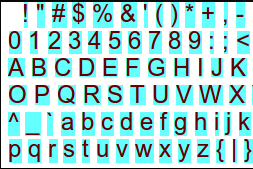
\includegraphics[width=0.8\textwidth]{Seg_example_1}
    \caption{Example 1}
\end{figure}

Dans le but de produire une série de caractères qui servirait de dataset pour entraîner le réseau de neurones, j'ai créé une variante de la segmentation : une fois qu'elle a découpé un caractère dans un rectangle elle coupe les bordures, la redimensionne puis sauvegarde l'image dans un dossier.

\newpage

Pour faire les histogrammes que j'utilise dans la fonction de suppressions des bordures, je prend en paramètre l'axe que je veux analyser et une liste dont la longueur est soit la hauteur, soit la largeur de l'image. Ensuite j'attribue aux cases d'indice i un entier correspondant aux nombres de pixels noirs trouvé sur la ligne/colonne d'indice i.

Bien que je n'ai finalement pas utilisé de fonction récursive basé sur l'algorithme \textit{recursive XY cut}, je voulais faire une fonction de découpage en bloc basé sur cet algorithme mais non récursif que j'aurais appelé une fois. Malheureusement le temps a finit par manquer et je n'ai pas pu faire cette fonction.

\section{Réseau neuronal (Antoine)}

Le réseau de neurones a été particulièrement difficile à mettre en place lors de cette deuxième partie du projet. En effet, les fonctions d'activations n'étaient pas les mêmes, j'ai essayé d'implémenter la fonction softmax pour activer la sortie. De plus, la quantité de données traitées, comparé au cas du réseau XOR, était très élevée. Le nombre de sorties a rendu difficile l'étape de \textit{Backpropagation}... Un vrai casse tête.

\begin{figure}[H]
    \centering
    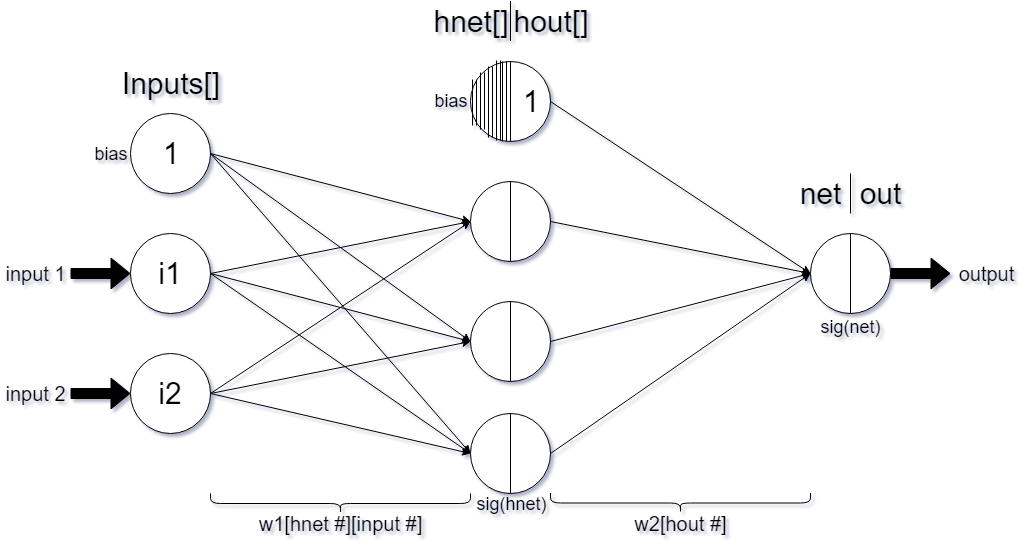
\includegraphics[width=1\textwidth]{XOR_Neural_Network}
    \caption{XOR neural network}
\end{figure}

Je vais ici réutiliser le shéma du réseau de neuronnes XOR, beaucoup plus compact que celui du réseau de l'OCR, afin de représenter visuellement un réseau de neurones.

\newpage

Le premier gros changement, comme mentionné ci-dessus, est le nombre d'entrées et de sorties. En effet, ce réseau traitant une image et non pas une comparaison entre deux nombres binaires, il est nécéssaire d'utiliser une entrée par pixel. Il se pose alors le problème de la complexité: il était dans un premier temps prévu d'utiliser des images de taille 28x28 pixels. Cependant, le réseau était vraiment lent, et il était difficile de lui faire apprendre même une quantité réduite de caractères de manière efficace. J'ai donc décidé de modifier cette taille en 10x10 pixels, passant alors de 784 à 100 entrées. Pour ce qui est du hidden layer, j'ai fini par paramétrer 71 neurones. Ce nombre est assez arbitraire, je me suis basé sur les conseils d'autres camarades s'occupant du réseau de neuronnes dans leur groupe. Ce nombre semble fonctionner, je l'ai donc laissé ainsi.

Le choix du nombre d'éléments à apprendre a également beaucoup évolué:

\begin{figure}[H]
    \centering
    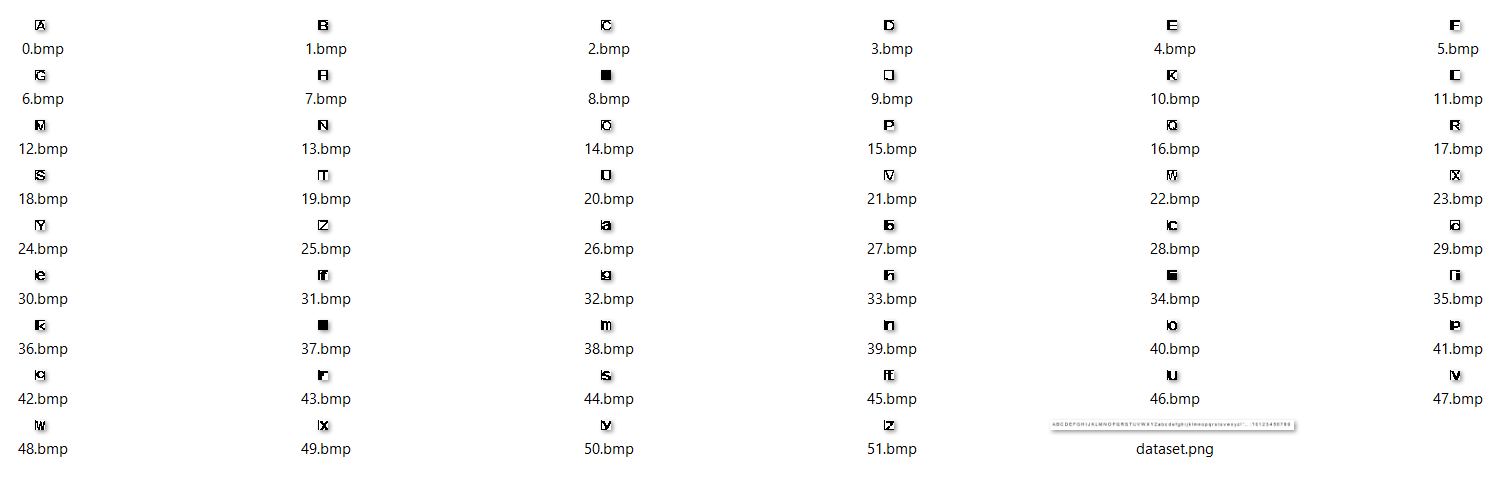
\includegraphics[width=1\textwidth]{dataset}
    \caption{Training dataset}
\end{figure}

\begin{figure}[H]
    \centering
    
\includegraphics[width=0.24\textwidth]{dataset_sample}
    \caption{One sample of the dataset}
\end{figure}

Lors de la première soutenance, ayant clairement sous-estimé la difficulté de ce projet, j'avais envisagé de faire apprendre l'alphabet (majuscule et minuscule) et les chiffres à notre réseau, sous forme manuscrite. Sauf qu'un problème m'a très rapidement fait changer de cap: nos exemples d'entrainement n'étaient pas à la bonne dimension, et nous ne disposions pas encore d'une segmentation fonctionnelle, ni suffisament rapide pour redimensionner des centaines de millier d'images, ou même une partie de ce dataset. J'ai donc réduit l'apprentissage du réseau à une police d'écriture, Arial, et j'ai décidé de finalement retirer les chiffres, afin de simplifier l'apprentissage: les caractères étant fortement redimensionnés, la perte de qualité pouvait rendre certains caractères presque identiques. Ce problème se pose encore aujourd'hui par exemple avec le 'z' majuscule et minuscule, ou le 'f' et le 't', mais selon les séquences d'entrainement, le réseau assimile correctement la plus grande partie de l'alphabet...

\begin{figure}[H]
    \centering
    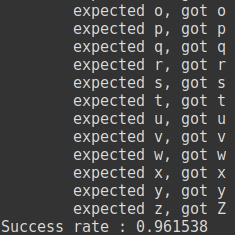
\includegraphics[width=0.7\textwidth]{training}
    \caption{Training results of one run}
\end{figure}

Mais il s'avère que le réseau semble malgré tout avoir des difficultés en situation réelle. Il se peut qu'il se soit contenté d'apprendre par coeur nos exemples d'entrainement, ou que quelques variations dans la segmentation d'un fichier réel l'induisent en erreur. Notre fonction de redimensionnement est aussi loin d'être idéale, déforme beaucoup les caractères et ajoute des bandes noires qui rejoignent les bords de l'image. Mais faute de temps, il a été impossible de corriger complètement ces lacunes avant le rendu final.

Enfin, dernier changement depuis la première soutenance: la structure de données. J'ai pendant longtemps (trop longtemps) essayé de maintenir le réseau sous forme de simples \textit{arrays}. 

\newpage

Cependant après des semaines de difficultés, des modifications importantes de ma représentation (remplacement des pointeurs par des tableaux, changement des matrices en tableaux une-dimension...) et une pression grandissante à l'approche de la date limite, j'ai décidé d'abandonner cette méthode (malgré son succès pour le XOR). Au lieu de contenir des tableaux pour les différentes valeurs à stocker, j'ai organisé le réseau de neurones en \textit{struct} 'Network', de même pour chaque neurone (que j'ai nommé 'Layer' car souvent manipulés par groupes). 

Chaque Network contient donc des Layers ainsi que leur taille respective, et chaque neurone contient diverses informations (sa valeur nette, sa valeur activée, ses poids et son bias, ainsi que ceux du tour précédent de l'entrainement). Ce choix fut long à mettre en place et à manipuler (de simples tableaux étant bien plus intuitifs), mais il a permis d'enfin obtenir un réseau fonctionnel capable d'apprendre.

Pour ce qui est de l'apprentisage et de l'évaluation d'une entrée, j'ai essayé différentes méthodes. J'ai utilisé dans un premier temps la fonction \textit{Sigmoid}, puis \textit{ReLU}, pour le hidden layer ; et j'ai tenté d'utiliser \textit{Softmax} pour la sortie. Avant de retourner à la case départ et d'utiliser \textit{Sigmoid} pour toutes les activations, car plus simple à dériver. J'ai également eu du mal à gérer la \textit{backpropagation}, ayant mis du temps à comprendre dans quel ordre calculer quels gradients, comment les assembler, et comment remonter l'information pour modifier les poids. C'est d'ailleurs le mauvais fonctionnement de cette correction qui m'a poussé à abandonner la représentation par tableaux de notre réseau de neurones.

\newpage

Pour conclure, la création de ce réseau neuronal aura été particulièrement difficile et frustrante. Mais nous avons fini par obtenir un réseau fonctionnel qui apprend l'alphabet suffisament bien pour nos attentes. 

\section{Interface utilisateur (Jérémy)}

Tout d’abord, je me suis intéressé au choix des bibliothèques qui constitueront notre interface. Nous avons choisi GTK+, développé à l’origine en C, pour sa portabilité. Afin d’interagir avec notre application, il nous faut créer une fenêtre. Le widget permettant d’afficher une fenêtre se nomme "GtkWindow". Les objets graphiques utilisent la notion d’héritage afin de récupérer des propriétés et des méthodes de widgets parents pour modifier leur propre comportement sans avoir à tout redéfinir. 

\begin{figure}[H]
    \centering
    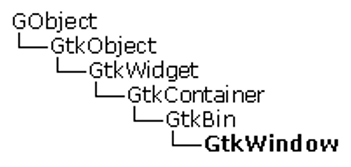
\includegraphics[width=0.5\textwidth]{GTK1}
    \caption{Windows inheritance with GTK}
\end{figure}

Ensuite, nous devions utiliser plusieurs éléments essentiels d’une interface graphique : les box et les boutons. GTK+ a certains avantages comme certains inconvénients. Nous ne pouvons pas intégrer plusieurs widgets dans une fenêtre car un "GtkContainer" ne peut en contenir qu’un seul. 

Pour résoudre ce problème, je me suis penché sur l’utilisation de deux catégories de "GtkBox" :

\begin{itemize}[label=\textbullet]
	\item Les \textbf{GtkHBox} qui permettent de disposer les widgets horizontalement
	\item Les \textbf{GtkVBox} qui permettent de les disposer verticalement
\end{itemize}

De plus, les boutons permettent à l’utilisateur d’effectuer une action grâce à un simple clic de souris. 

\begin{figure}[H]
    \centering
    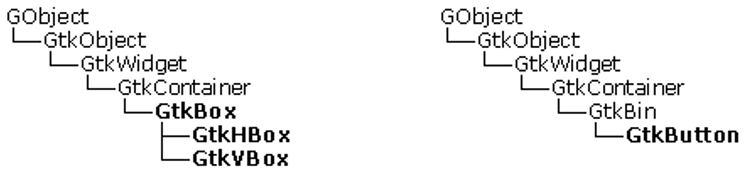
\includegraphics[width=1\textwidth]{GTK2}
    \caption{Boxes and buttons inheritance with GTK}
\end{figure}

Pour cela, j’ai étudié le fonctionnement des signaux afin que ceux-ci ne se terminent qu’au moment où l’utilisateur le demande. Lorsque l’utilisateur interagit avec l’application, le widget concerné émet un signal. Il est associé à une ou plusieurs significations et permet donc de programmer toutes les actions possibles. J’ai donc créé plusieurs fonctions "callback" qui connectent le signal au bouton concerné. 

\newpage

L'OCR s'utilise donc en utilisant les fonctions suivantes dans l'ordre (les cinq premières s’activent avec le signal "clicked"):

\begin{itemize}[label=\textbullet]
	\item Ouvrir une image (qui ouvre une boite de dialogue standard pour sélectionner un fichier)
	\item Convertir l'image en texte
	\item Sauvegarder le texte convertit dans le répertoire de l'image
	\item Le sauvegarder à nouveau si des modifications ont été effectuées sur le texte
	\item Fermer la zone de texte
	\item Quitter l'application (avec le signal "destroy")
\end{itemize}

J’ai également inclus une barre de défilement pour que le texte converti ne soit pas bloqué par une taille fixe de la zone de texte.

Enfin, nous avons rajouté à l’interface notre touche personnelle. Lorsque nous lancerons l’application, une fenêtre apparaitra montrant un « avant-gout » de ses capacités. Nous pouvons y remarquer l’identité des créateurs de l’OCR comme ci-dessous.

\begin{figure}[H]
    \centering
    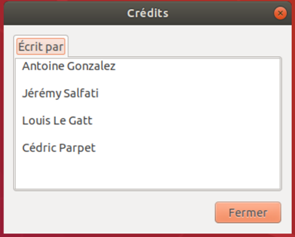
\includegraphics[width=0.5\textwidth]{credits}
    \caption{Credits}
\end{figure}

Tout cela nous donne l'interface graphique suivante:

\begin{figure}[H]
    \centering
    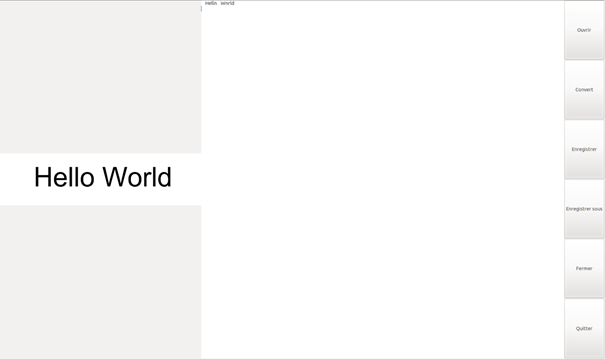
\includegraphics[width=0.9\textwidth]{UI_2}
    \caption{Current user interface}
\end{figure}

\chapter{Difficultés rencontrées}

\section*{Traitement de l'image}

Les premières difficultés ont été dans l’apprentissage du langage C, et surtout de l’éditeur de texte Vim. L’apprentissage et la prise de différentes habitudes sur Vim a été une partie assez complexe. J’ai essayé d’installer une certaine quantité de plugin afin de faciliter l’utilisation de cet éditeur et d’améliorer mon efficacité pour coder. Une fois ces difficultés dépassées et les premiers travaux pratiques réalisés j’ai eu un réel déclic sur la manière de coder et d’organiser mon code. En effet j’ai très vite vu qu’il était indispensable d’organiser son code, de le commenter et de le séparer dans différents fichiers logiques les différentes parties du code.

J’ai aussi rencontré des difficultés pour essayer de rendre possible l’utilisation de la fonction « anti bruit » sans succès car je n’ai pas réussi à rendre le texte sur l’image lisible par le réseau de neurones après passage dans la cette fonction. Cependant je reste content d’avoir réussi à implémenter cette fonction. Concernant SDL, les principales difficultés ont été liées à la compréhension de la bibliothèque et surtout au manque de documentation sur ses fonctions.

\section*{Segmentation de l'image}

Tout au long du projet je me suis heurté à de nombreux problèmes. Même si au début j'avais déjà une idée de l'implémentation de la segmentation il m'a fallu apprendre à utiliser correctement la bibliothèque SDL et trouver les fonctions dont j'avais besoin. De manière plus générale, la maîtrise du C était essentiel pour ce projet et l'apprendre était donc une obligation mais aussi une épreuve en soit. La création d'un Makefile m'a également posé des difficultés au début. 

J'ai dû beaucoup chercher pour trouver pourquoi une fonction récursive pouvait être une bonne idée, et j'ai passé beaucoup de temps à essayer d'implémenter cela, malheureusement sans succès. Je rencontrais non seulement des problèmes au niveau du code mais aussi d'un point de vue théorique. La fonction que j'imaginais ne pouvait par exemple pas découper un texte correctement si elle trouvait un espace sans pixels noirs en plein milieu du texte. Comme par exemple si on répétait la même phrase sur plusieurs lignes, les espaces coïncideraient et la segmentation aurait coupé en plein milieu de la phrase. 

L'utilisation de gdb pour débuguer a été une épreuve supplémentaire car cet outil n'est vraiment pas facile à utiliser. 

Enfin je pense que l'une des plus grosses épreuves que j'ai du rencontrer était le temps. Pour ce projet nous n'avions pas de semaine de libre avant les rendus et cela nécessitait donc de faire tout le projet en plus des cours. C'est peut-être pour moi la plus grosse épreuve et probablement la première à surmonter d'un projet dans ces conditions.

\section*{Réseau neuronal}

Comme évoqué dans le détail de cette partie dans les pages précédentes, cette partie a été très difficile à mettre en place. Elle avait déjà été compliquée avec le XOR, mais le réseau du programme final a dépassé toutes mes attentes en matière de frustration.

Cette difficulté est en grande partie due au manque de ressources pour les réseaux de neurones utilisant le langage C. En effet, la majorité des ressources utilisent Python, qui dispose de bibliothèques facilitant grandement le travail, et surtout de beaucoup moins de contraintes d'usage de types. Même au sein des ressources généralisées, les explications sont souvent maladroites, difficiles à comprendre, voire même fausses. Certaines étapes sont parfois omises, les formules ne sont pas les mêmes d'un utilisateur à l'autre... Autrement dit, l'internet n'a pas été aussi instructif qu'à son habitude, et il a fallu chercher pendant longtemps et demander de l'aide à beaucoup de monde avant de réussir à implémenter mon réseau. Cette aide n'a pas été facile à obtenir non plus. En effet, en général, seul un membre par groupe de projet s'occupe du réseau de neurones, donc seulement un quart (ou moins, n'étant pas le seul à avoir des difficultés) de mes collègues étaient véritablement capable de m'aider. Et chaque personne procédant à sa propre manière, les quelques explications que je pouvais récolter n'étaient pas toujours applicables à mon cas.

Enfin, après avoir finalement réussi à implémenter le réseau, il a fallu ajuster les paramètres de ce dernier (constante d'apprentissage, momentum, nombre de neurones de la couche cachée...), étape particulièrement aléatoire car il n'existe pas de règle générale pour choisir ces paramètres. 

\newpage

Cela ne pose pas de problème lorsque le réseau apprend en quelques secondes comme actuellement. Mais étant donné son optimisation inexistante pendant longtemps, cette étape d'essayer en boucle en ajustant les paramètres petit à petit était particulièrement longue lorsque le réseau mettait une, deux, voire cinq secondes afin de réaliser une seule \textit{backpropagation}.

Vous l'aurez compris, cette partie de l'OCR n'aura pas été la plus agréable. Néanmoins la satisfaction d'obtenir un réseau capable d'apprendre reste une très belle récompense.

\section*{Interface utilisateur}

Concernant l’interface graphique, j’ai eu de nombreuses difficultés que j’ai réussi à surmonter. 
En effet, je devais intégrer correctement deux box (l’une étant la zone d’image, l’autre, l’emplacement des boutons) dans un conteneur (appelé "main\_box") qui lui-même se trouve dans une fenêtre. Le tout rendait finalement notre application intuitive.

De plus, je pensais qu’il fallait contenir un widget image dans une zone de texte. Je me suis rendu compte que ce n’était pas la bonne solution après quelques jours, me tournant vers une option plus pragmatique : créer une nouvelle box.

Mes principales épreuves étaient surtout l’apprentissage rapide et efficace du langage C et le fait de relier mon travail à celui des autres membres. En effet, j’utilise dans l’interface des listes chainées, évidemment des pointeurs et la notion d’héritage via GTK+. 

\newpage

D’autre part, j’ai eu une véritable difficulté à concevoir la fonction "callback" permettant la conversion d’une image en un document texte. Je ne trouvais pas dans la bibliothèque, de lien entre SDL ("SDL\_Surface") et GTK+ ("GtkWidget") tout simplement parce qu’il n’y en a pas ! Après de longues recherches sur la manière dont créer ce signal, j’ai enfin trouvé une fonction dans la librairie de SDL, appelée "IMG\_Load" prenant en paramètre le fichier "filename".


\chapter{Expériences personnelles}

\begin{itemize}
	\item \textbf{Louis :} Ce projet a été une vraie épreuve. En effet il a fallu apprendre énormément seul, que ce soit pour le langage C ou pour apprendre à utiliser la bibliothèque SDL, très importante pour ma partie. Cependant il m’a permis de me pousser à faire énormément de recherche dans divers domaines et à comprendre comment fonctionne des algorithmes pour les implémenter ensuite en C pour notre OCR. De plus ce projet m’a donné une vision différente du travail en équipe et m’a permis d’être très autonome sur ma partie. En effet le découpage du projet étant très claire entre les différents membres du groupe il fallait que chacun d’entre nous soit à la hauteur du travail à réaliser afin de ne pas provoquer de retard sur les parties des autres membres. J’ai de plus pu comprendre le fonctionnement d’un logiciel. De l’imagination de celui-ci à sa conception et à sa finalisation. Je n’avais aucune idée des différentes phases de développement ni du temps que celle-ci prendrai. Ce projet me permet donc d’avoir une idée plus précise du temps qu’il faut pour créer entièrement une application de ce style.
\end{itemize}

\newpage

\begin{itemize}
	\item \textbf{Cédric :} Ce projet aura été un défi et une expérience intense du début jusqu'à la fin et particulièrement sur la fin. Comme pour celui de l'année précédente ce projet m'aura montré l'importance de la coordination dans un projet en équipe et la nécessité de bien se documenter pour mieux maîtriser des outils qui m'étaient inconnus avant. Il m'aura surtout montré, encore plus que le projet précédent, l'importance de travailler sur la durée et en plus des cours.
\end{itemize}
\begin{itemize}
	\item \textbf{Antoine :} Ce projet aura été une expérience très intéressante. Beaucoup moins ludique que le projet de première année, et beaucoup moins libre, il était cependant très intéressant. Les réseaux de neurones étaient pour moi incompréhensibles il y a encore quelques mois. Et pour être honnête, ils le sont encore un peu, mais beaucoup moins, et je suis très heureux d'avoir pu apprendre à en créer un. Le sujet général était très intéressant car il est facile d'imaginer une application réelle à un tel programme, et les resrictions ainsi que l'absence de semaines "dédiées" au projet permettent de mieux se préparer à un cadre plus professionel, où les deadlines sont moins espacées et les restrictions sont nombreuses. Enfin, il est toujours très satisfaisant de voir son projet prendre vie au fur et à mesure que le groupe progresse: en partant d'un simple cahier des charges et de connaissances limitées voire inexistantes dans les domaines nécéssaires à sa réalisation, nous avons pu obtenir un programme fonctionnel correspondant aux attentes de chacun. La plannification et l'organisation reste de loin l'étape que je préfère, et après les nombreuses frustrations liées à ma partie, je sais désormais que si j'ai le choix, je n'utiliserai pas C pour réaliser de réseau de neurones, si j'en réalise encore. Malgré tout, bien que notre réseau de neurones soit loin de la géniale intelligence artificielle dont je rêvais, je suis malgré tout très heureux d'avoir pu créer cette version moins sofistiquée mais qui se débrouille malgré tout relativement bien.

\end{itemize}
\begin{itemize}
	\item \textbf{Jeremy :} Tout au long de ce deuxième projet informatique, j’ai pu acquérir de nombreuses notions essentielles en programmation : la prise en main du langage C, les pointeurs, les listes chainées, la notion d’héritage via GTK+ concernant les widgets et les boutons… Je tiens à repréciser que j’ai pu apprendre à coder en C plus rapidement dans ce contexte qu’en travaux pratiques. Également, un tel projet ne peut qu’être bénéfique et très intéressant dans la construction de mon parcours d’ingénieur. Mes parents ne sont que plus que surpris et fiers de leur fils lorsqu’il constatent ma progression en code et surtout le résultat obtenu. Même si j’ai dû affronter certaines difficultés lors de mon avancement, je peux actuellement vous montrer que je les ai dépassées par une véritable interface graphique intuitive et fonctionnelle.
\end{itemize}

\chapter{Conclusion}

Ce projet touche à sa fin. Ces quelques mois de travail ont fini par porter leurs fruits, malgré les très nombreuses difficultés rencontrées.

Chaque membre du groupe a mené à bien la partie qui lui était attribuée, et nous avons pu progresser avec fluidité sans problème de communication entre les membres, ni réel problème d'interactions entre les parties. Cela a été une très bonne expérience pour chacun, et cela nous a permis de nous former à de nouveaux concepts jusqu'alors inconnus pour nous. Malgré la difficulté d'utiliser le langage C, langage bas niveau et avec la restriction d'une norme plus ancienne, et l'hostilité de certaines ressources utilisées (GTK+ et SDL), nous avons fini par obtenir le programme attendu.

Nous disposons désormais d'un OCR capable de reconnaitre l'alphabet en majuscule et minuscule avec une police d'écriture très courante. 

Le programme n'est pas parfait, bien évidemment. Tout est perfectible. Mais nous sommes très satisfait du résultat obtenu pour une première expérience avec tous les concepts abordés lors de sa conception.

\chapter{Bibliographie}

\section*{Louis}

\begin{itemize}
	\item \textit{http://www.f-legrand.fr/scidoc/docimg/numerique/filtre/median/median.html}
	\item \textit{https://www.libsdl.org/}
	\item \textit{https://openclassrooms.com/fr/courses/19980-apprenez-a-programmer-en-c/17117-installation-de-la-sdl}
\end{itemize}

\section*{Jérémy}

\begin{itemize}
	\item \textit{https://gtk.developpez.com/cours/gtk2/}
	\item \textit{https://nicolasj.developpez.com/gtk/cours/}
	\item \textit{https://www.gtk.org/documentation.php}
	\item \textit{https://openclassrooms.com/fr/courses/1387611-creez-une-interface-avec-gtk}
\end{itemize}

\section*{Antoine}

\begin{itemize}
	\item \textit{https://deepnotes.io/softmax-crossentropy}
	\item \textit{https://medium.com/\@14prakash/back-propagation-is-very-simple-who-made-it-complicated-97b794c97e5c}
	\item \textit{https://medium.com/datathings/neural-networks-and-backpropagation-explained-in-a-simple-way-f540a3611f5e}
	\item \textit{http://neuralnetworksanddeeplearning.com/chap2.html}
	\item \textit{https://stats.stackexchange.com/questions/235528/backpropagation-with-softmax-cross-entropy}
	\item \textit{https://www.youtube.com/playlist?list=PLZHQObOWTQDNU6R1\_67000Dx\_ZCJB-3pi}
\end{itemize}

\section*{Cédric}

\begin{itemize}
	\item \textit{"A Modified Recursive X-Y Cut Algorithm for Solving Block Ordering Problems"}, par Phaisarn Sutheebanjard et Wichian Premchaiswadi
	\item \textit{"Optimized XY-Cut for Determining a Page Reading Order"}, par Jean-Luc Meunier
	\item \textit{http://erik.deblan.org/blog/index.php?article13/c-que-faire-en-cas-de-segmentation-fault}
	\item \textit{http://www.delafond.org/traducmanfr/man/man1/gdb.1.html}
	\item \textit{https://wiki.libsdl.org/}
	\item \textit{https://en.wikipedia.org/wiki/Recursive\_XY-cut}
\end{itemize}

\vfill

\end{document}
